\documentclass{article}
\usepackage{algorithm, algpseudocode}
\usepackage{amsmath, amssymb, amsthm}
\usepackage{color}
\usepackage{enumerate}
\usepackage{geometry}
\usepackage{graphicx}
\usepackage{hyperref}

\newcommand{\problem}[1]{\textsc{#1}}

% Create theorem environments as needed
\newtheorem{lemma}{Lemma}
\newtheorem{theorem}{Theorem}
\newtheorem{definition}{Definition}
\newtheorem*{observation}{Observation}

\usepackage{tabularx}
\newcommand{\defproblem}[4]{%
  \hfill\\\smallskip\noindent%
  \begin{tabularx}{\textwidth}{|l X|}%
    \hline%
    \multicolumn{2}{|l|}{\problem{#1}}\\%
    \textbf{Input:}&#2\\%
    \textbf{Parameter:}&#3\\%
    \textbf{Question:}&#4\smallskip\\\hline%
  \end{tabularx}%
  \smallskip%
}%
\newcommand{\proofnewline}{\mbox{}\\*}

\title{Proof Review Exercise \#1}
\begin{document}
\maketitle

\section*{Week-2}
\subsection*{Background}

\defproblem{$k$-MaximalMatching}
{A graph $G = (V,E)$ and a non-negative integer $k$}
{$k$}
{Does $G$ have a maximal matching of size at most $k$?}

\subsection*{Main Result}

\begin{theorem}
There is a $O(k^2)$ kernel for \problem{$k$-MaximalMatching}.
\end{theorem}

\begin{proof} Denote our graph by $G$. \\

\noindent \emph{High-level strategy}: We will first relate maximal matchings to vertex cover, which gives us a notion of ``high-degree vertices.'' We will then use these vertices to identify ``useless'' vertices that can be safely removed from the graph. After applying this reduction method, we will reason that we are left with a $O(k^2)$ kernel.\\

\noindent \emph{Reduction methods and safeness}: Note that every maximal matching can be turned into a vertex cover by taking both endpoints of every matched edge -- if not, there exists some uncovered edge not in the matching, which contradicts the maximality of our matching. Therefore, if we hope to get a maximum matching of size at most $k$, we also hope that an optimal vertex cover for this graph has size at most $2k$. Using this fact, let $X$ be the set of vertices whose degree is at least $2k+1$. We know that each vertex in $X$ must be an endpoint of a matched edge, otherwise all of its neighbors must be endpoints of matched edges, which cannot be done with a matching of size at most $k$.

While we have identified this set of ``high-degree vertices,'' we cannot directly remove them from the graph. Specifically, we know each high-degree vertex is an endpoint of a matched edge, but we don't actually know \emph{which} edge. Instead, we will use $X$ to derive another reduction. Examine the graph $G \setminus X$, and let $v$ be an isolate in this graph (if one exists). We know that the neighbors of $v$ must be high-degree vertices (which are endpoints of matched edges), therefore we know that we would never add an edge incident to $v$ to our maximal matching. In general, then, we may remove all isolated vertices in $G \setminus X$ from $G$. See Figure \ref{figure:problem1} for a visualization.

\begin{figure}
\label{figure:problem1}
\begin{center}
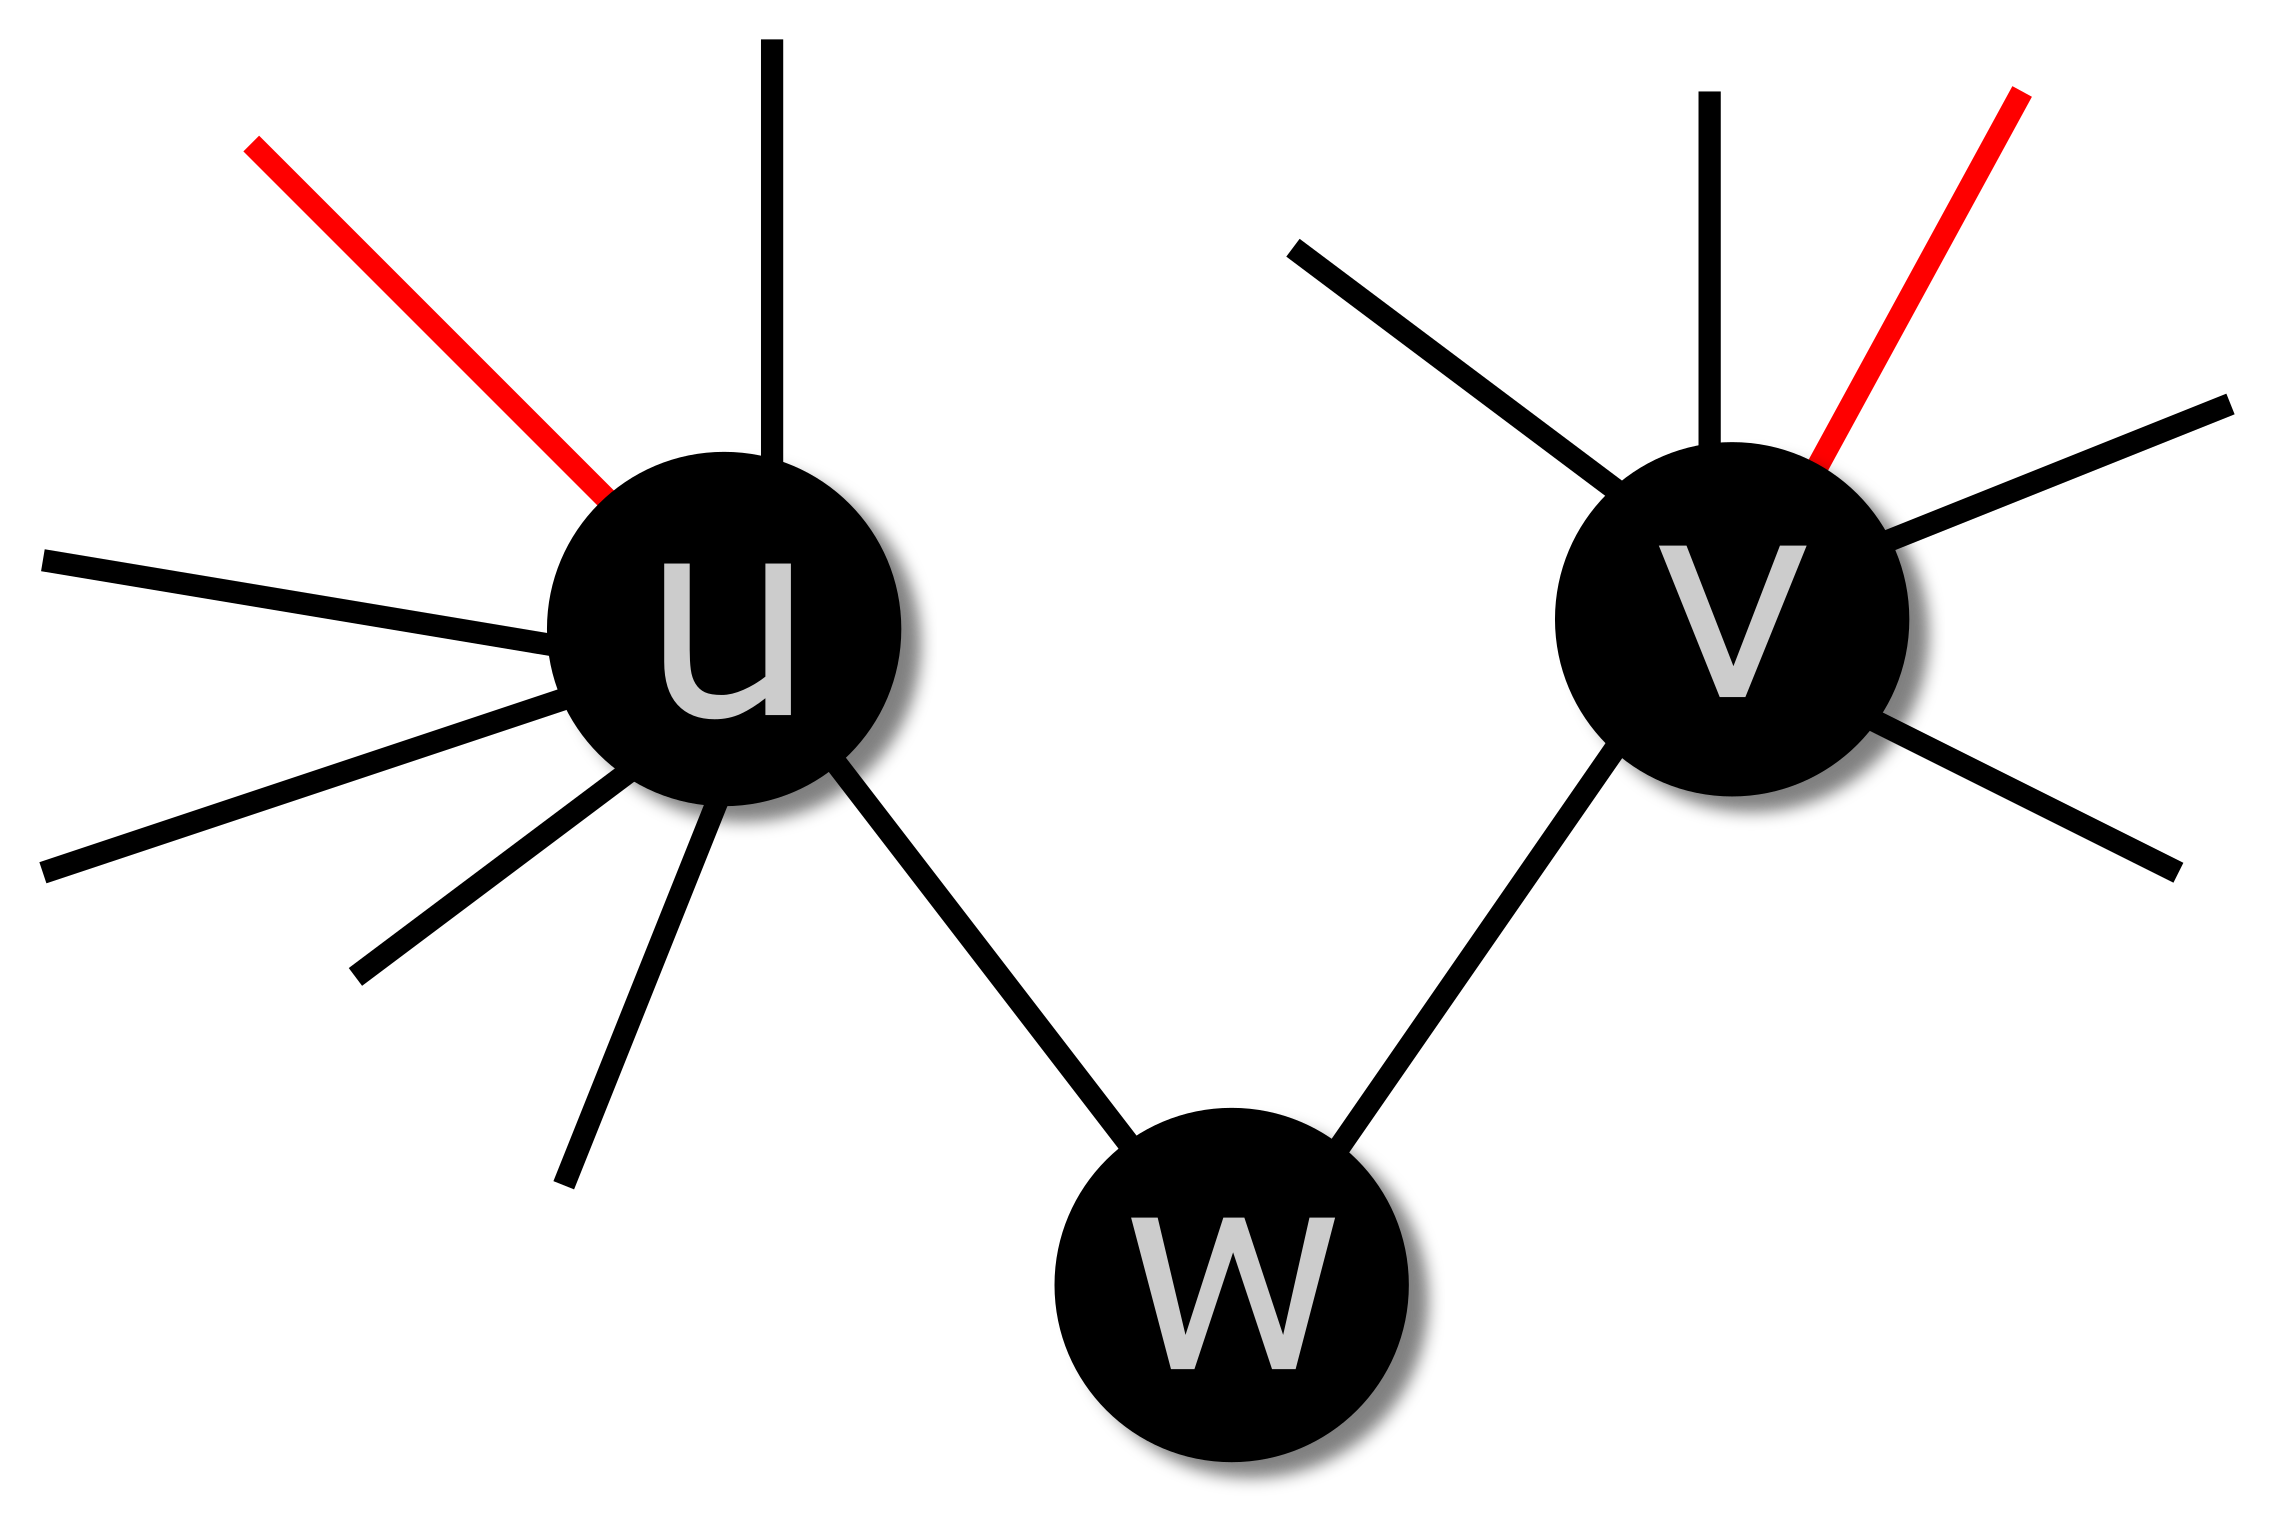
\includegraphics[width=0.4\textwidth]{frame1}
\hspace{0.15\textwidth}
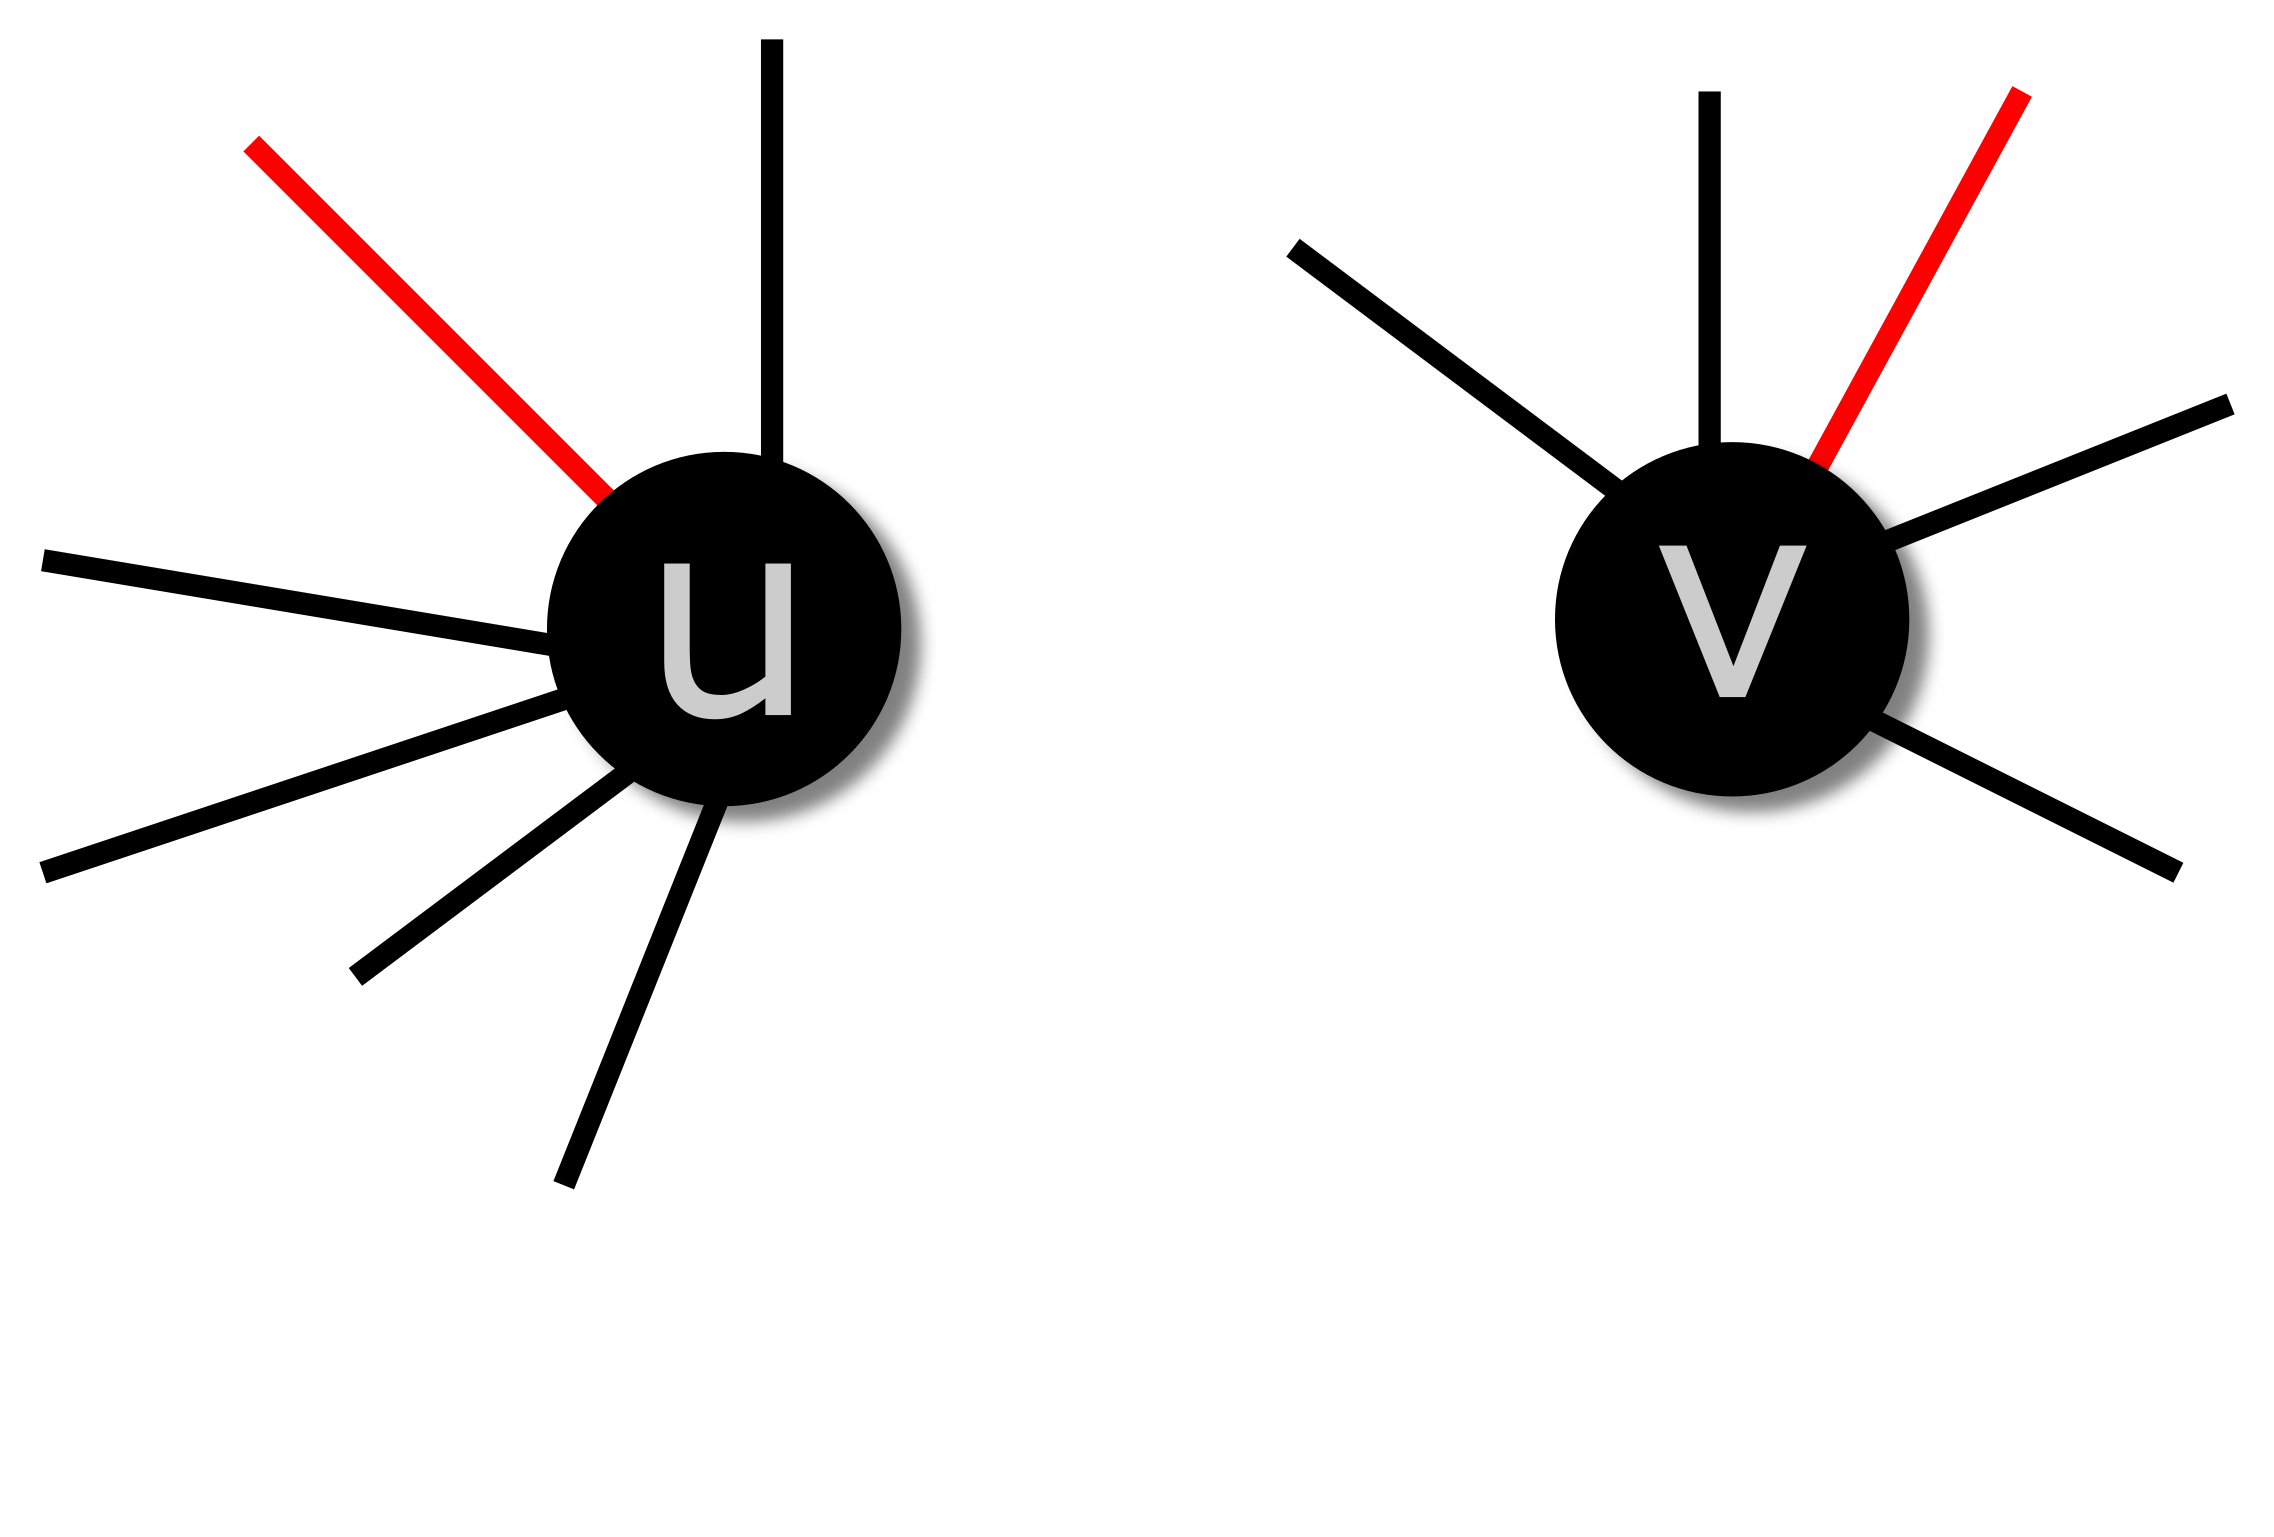
\includegraphics[width=0.4\textwidth]{frame2}
\end{center}
\caption{(Left) Let $u$ and $v$ be two high-degree vertices. Because of how we defined ``high-degree,'' we know that $u$ and $v$ must be endpoints of matched edges, shown in red. (Right) If $w$ is only connected to $u$ and $v$ then we can remove $w$ from the graph. This is safe because if the edge $(u, w)$ (or $(v, w)$) was in the matching, then we simply add an edge incident to $u$ (or $w$) to the matching -- this guarantees that $u$ (or $w$) is still covered.}
\end{figure}

\newpage
Formalizing this discussion, we define the following two reduction methods:
\begin{enumerate}[\text{RR}1.]
\item Identify the set of vertices with degree at least $2k+1$. Denote this set $X$. Do not remove $X$ from $G$, merely identify them.
\item Identify the set of isolated vertices in $G / X$ and remove them from $G$.
\end{enumerate}

\noindent \emph{Run time}: Identifying the set of high-degree vertices $X$ will take $O(n^2)$ if the graph is stored as an adjacency matrix. Identifying the isolates of $G \setminus X$ will also take $O(n^2)$. Therefore both reduction routines execute in $O(n^2)$ time.\\

\noindent \emph{Output bound}: First, we know that $|X| \leq 2k$, otherwise we'd have enough vertices to pair off to get a maximal matching larger than $k$. Second, in a \texttt{YES}-instance, the graph $G \setminus X$ is bounded by $4k^2$. By the second rule and the fact that we have a \emph{maximal} matching, we know that every vertex must be an endpoint of a matched edge. There are at most $k$ such edges, each of whose endpoints can have degree at most $2k$, therefore there are at most $4k^2$ vertices in $G \setminus X$. In total, then, the produced instance has at most $O(k^2)$ vertices.
\end{proof}

\newpage
\section*{Week-3}
\subsection*{Background}
\begin{definition}
A graph is \emph{perfect} if, for every induced subgraph, the clique number is equal to the chromatic number.
\end{definition}

\begin{definition}
We denote an induced cycle on three vertices as a \emph{triangle}. A graph is \emph{triangle-free} if it does not contain a triangle.
\end{definition}

\begin{definition}
Let $G = (V, E)$ be a graph. An \emph{odd cycle transversal} $S \subseteq V$ is a set of vertices such that $G \setminus S$ is bipartite.
\end{definition}

\defproblem{$k$-OCT}
{A graph $G = (V,E)$ and a non-negative integer $k$}
{$k$}
{Does $G$ have an odd cycle transversal of size at most $k$?}

\subsection*{Main Result}
\begin{lemma}
\label{lemma:perfect}
A perfect graph is bipartite if and only if it is triangle-free.
\end{lemma}
\begin{proof}\proofnewline
\emph{Forward direction}: Assuming that $G$ is perfect and bipartite, we will show that it is triangle-free. Suppose not, and there exists an induced triangle on vertices $u, v, w$. Since $G$ is perfect and the triangle is a 3-clique, $G$ must have chromatic number at least 3. But this contradicts the assumption that $G$ is bipartite, since every bipartite graph is 2-colorable (e.g. use a unique color per partite set).\\

\noindent \emph{Backwards direction}: Assuming that $G$ is triangle-free and perfect, we will show that it is bipartite. Since $G$ is triangle-free, it cannot contain a clique larger than $K_2$. We split into two cases:
\begin{enumerate}[\text{Case} 1.]
\item $G$ has no edges. Then $G$ is trivially bipartite -- put every vertex in one partite set.
\item $G$ has an edge. Then by the assumption that $G$ is perfect and the fact that its largest clique is $K_2$, it has a 2-coloring. This coloring implies a bipartite construction -- have a partite set per color.
\end{enumerate}
In all cases, $G$ is bipartite.
\end{proof}

\begin{theorem}
\problem{$k$-OCT} has a $3^k n^{O(1)}$ branching algorithm in perfect graphs.
\end{theorem}
\begin{proof}
\proofnewline

\noindent \emph{High-level strategy}: Using the previous lemma, we know that we need to break every triangle to make the graph bipartite. We know that every triangle contains a vertex in an optimal OCT set, but we don't know which one to add -- so we will branch!\\

\noindent \emph{Algorithm description}: Define a recursive method that takes as input a graph $G$, a parameter $k$, and a (partial) OCT set $S$. Go through all triples of vertices $u, v, w$ until a triangle is found. If a triangle is found, then branch into three subproblems -- one where $u$ is added to $S$, one where $v$ is added to $S$, and one where $w$ is added to $S$; in all cases remove the vertex from $G$ and decrease $k$ by one when recursing. If a triangle is not found, then return \texttt{YES} if $k \geq 0$, and \texttt{NO} otherwise.\\

\noindent \emph{Correctness}: We terminate when no triangle could be found, so the graph is bipartite (by Lemma \ref{lemma:perfect}) and $S$ is a valid OCT set. If $k \geq 0$ then we know that $|S| \leq k$ and the solution should be \texttt{YES}. Likewise, if $k < 0$ then we know that $|S| > k$ and the solution should be \texttt{NO}. Therefore our algorithm always constructs a valid OCT set, and correctly decides if it is too large or not.\\

\noindent \emph{Run time}: Enumerating all triples of vertices takes $\binom{n}{3} = O(n^3)$ time, and checking if a triple is a triangle takes $O(1)$ time if we store the graph with an adjacency matrix. Examining $k$ to decide \texttt{YES} or \texttt{NO} takes $O(1)$ time, so each node of the branching tree takes $O(n^3)$ time to execute. Every time we branch we decrease $k$ by exactly 1, therefore the branching tree has depth $k$. Additionally, we always branch into three subproblems, therefore there are at most $O(3^k)$ nodes in the branching tree. In total, then, the run time is $O(3^kn^3)$.
\end{proof}

\begin{observation}
Note the similarities to the $O(k^2)$ kernel for \problem{$k$-ClusterEdit}! Would you expect to also get a $O(k^2)$ kernel for \problem{$k$-OCT}? Would you expect to get a $3^k n^{O(1)}$ branching algorithm for \problem{$k$-ClusterEdit}?
\end{observation}

\newpage
\section*{Week-4}
\subsection*{Background}

\begin{definition}
Let $G = (V, E)$ be a graph. A \emph{feedback vertex set} $S \subseteq V$ is a set of vertices such that $G \setminus S$ is a forest (e.g. every cycle (``feedback loop'') is broken).
\end{definition}

\begin{definition}
Let $G = (V, E)$ be a graph. A \emph{dominating set} $S \subseteq V$ is a set of vertices such that, for all vertices $v \in V$, either $v \in S$ or $v$ has a neighbor in $S$.
\end{definition}

\defproblem{$k$-DominatingSet}
{A graph $G = (V,E)$ and a non-negative integer $k$}
{$k$}
{Does $G$ have a dominating set of size at most $k$?}

\subsection*{Main Result}
\begin{theorem}
There is an FPT algorithm for $k$-dominating set parameterized by feedback vertex set.
\end{theorem}

\begin{proof} Denote our graph by $G$.\\

\noindent \emph{High-level strategy}: NP-hard problems typically are easy on trees, so we will start by removing the feedback vertex set and solving dominating set on the remaining tree. We will then brute-force all ways of merging the feedback vertex set into the tree, which is fast given that the feedback vertex set is small.\\

\noindent \emph{Algorithm description}: Let $F$ be our feedback vertex set and $D$ be our (initially-empty) dominating set. By definition, $G \setminus F$ is a tree. We can use a ``dynamic programming''-style approach to compute an optimal dominating set: Starting from the leaves, check whether it is better to have a vertex or one of its (possibly-non-existent) children in a dominating set. At this point we have an optimal dominating set, but only for the tree $G \setminus F$. We now test every way of merging $F$ into this solution using brute force over $F$. If it was possible to finish the dominating set for $G$ with $|D| \leq k$ then output \texttt{YES}, otherwise output \texttt{NO}.\\

\noindent \emph{Correctness}: We check every possible dominating set on the feedback vertex set, there are no other options here. Everything else must live on a tree and we can compute the exact answer here, so a solution of size at most $k$ will always be found if it exists, and otherwise we answer \texttt{NO}.\\

\noindent \emph{Run time}: Computing the exact dominating set on the tree takes at most $O(n)$ time if we start from the leaves and ascend up the tree. Computing all dominating sets of the feedback vertex set takes time $\binom{n}{k} = O(n^k)$, which is a polynomial since $k$ is a constant. Therefore the full algorithm takes $O(n^k n) = O(n^{k+1})$ time.
\end{proof}
\end{document}
